
\begin{figure}
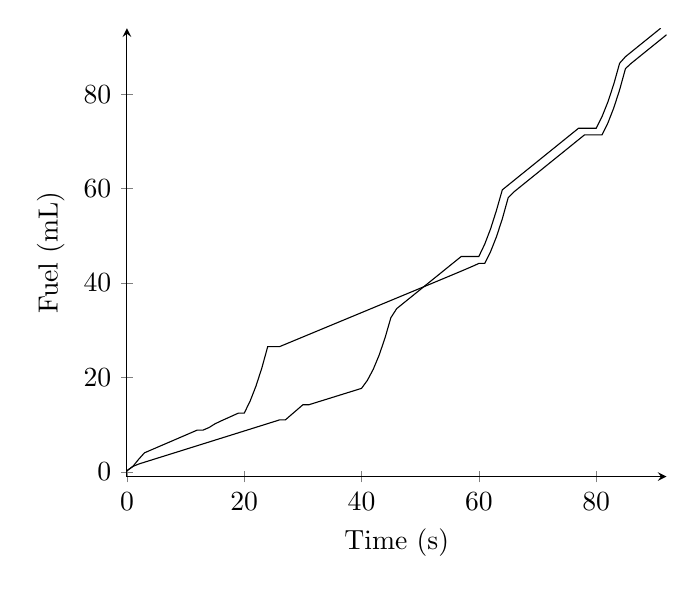
\begin{tikzpicture}
\begin{axis}[
legend style={
	anchor=west
},
axis x line=bottom,
axis y line=left,
ymin=-1,
point meta=explicit symbolic,
xlabel=Time (s),
ylabel=Fuel (mL)
]
\addplot[] coordinates {
(0, 0.239885513361)
(1, 1.13183007041)
(2, 1.65480786762)
(3, 2.0435945225)
(4, 2.43239638586)
(5, 2.82121469483)
(6, 3.21005082406)
(7, 3.59890630532)
(8, 3.98778285057)
(9, 4.3766823792)
(10, 4.76560705036)
(11, 5.1545593015)
(12, 5.5435418946)
(13, 5.9325579719)
(14, 6.32161112357)
(15, 6.7107054702)
(16, 7.09984576442)
(17, 7.48903751649)
(18, 7.87828715137)
(19, 8.26760220622)
(20, 8.65699158161)
(21, 9.04646586383)
(22, 9.43603774326)
(23, 9.82572256392)
(24, 10.2155390549)
(25, 10.6055103181)
(26, 10.9956651844)
(27, 10.9956651844)
(28, 12.0714773379)
(29, 13.1401452178)
(30, 14.2090813271)
(31, 14.2090813271)
(32, 14.5952560353)
(33, 14.9814463469)
(34, 15.3676579086)
(35, 15.7538995079)
(36, 16.1401856815)
(37, 16.5265425809)
(38, 16.9130234733)
(39, 17.2997619659)
(40, 17.6872817881)
(41, 19.394030385)
(42, 21.7378927219)
(43, 24.7228480645)
(44, 28.3593289432)
(45, 32.6642211535)
(46, 34.5861919733)
(47, 35.5901818363)
(48, 36.5941716994)
(49, 37.5981615624)
(50, 38.6021514254)
(51, 39.6061412884)
(52, 40.6101311515)
(53, 41.6141210145)
(54, 42.6181108775)
(55, 43.6221007405)
(56, 44.6260906035)
(57, 45.6300804666)
(58, 45.6300804666)
(59, 45.6300804666)
(60, 45.6300804666)
(61, 48.2333619131)
(62, 51.4811935161)
(63, 55.3866276288)
(64, 59.7448267459)
(65, 60.748816609)
(66, 61.752806472)
(67, 62.756796335)
(68, 63.760786198)
(69, 64.764776061)
(70, 65.7687659241)
(71, 66.7727557871)
(72, 67.7767456501)
(73, 68.7807355131)
(74, 69.7847253762)
(75, 70.7887152392)
(76, 71.7927051022)
(77, 72.7966949652)
(78, 72.7966949652)
(79, 72.7966949652)
(80, 72.7966949652)
(81, 75.2613741104)
(82, 78.3686254288)
(83, 82.1301026455)
(84, 86.5639127502)
(85, 87.9593727377)
(86, 88.9633626007)
(87, 89.9673524638)
(88, 90.9713423268)
(89, 91.9753321898)
(90, 92.9793220528)
(91, 93.9833119159)
};
\addplot[] coordinates {
(0, 0.239885513361)
(1, 1.13183007041)
(2, 2.66515136892)
(3, 4.03763383906)
(4, 4.57164172015)
(5, 5.10578751033)
(6, 5.64010132275)
(7, 6.17462244404)
(8, 6.70940302947)
(9, 7.24451370657)
(10, 7.78005232835)
(11, 8.31615812381)
(12, 8.85303551456)
(13, 8.85303551456)
(14, 9.3873411108)
(15, 10.1633948282)
(16, 10.7581034568)
(17, 11.3176767072)
(18, 11.8775088749)
(19, 12.4379781647)
(20, 12.4379781647)
(21, 14.9774570018)
(22, 18.1605383165)
(23, 21.9996309817)
(24, 26.5135971352)
(25, 26.5135971352)
(26, 26.5135971352)
(27, 27.0292868029)
(28, 27.5449771957)
(29, 28.060668386)
(30, 28.5763604561)
(31, 29.0920535)
(32, 29.6077476251)
(33, 30.123442955)
(34, 30.6391396326)
(35, 31.1548378239)
(36, 31.6705377229)
(37, 32.1862395574)
(38, 32.7019435969)
(39, 33.2176501619)
(40, 33.7333596374)
(41, 34.2490724883)
(42, 34.7647892821)
(43, 35.2805107174)
(44, 35.7962376639)
(45, 36.3119712162)
(46, 36.8277127709)
(47, 37.3435708273)
(48, 37.8597074822)
(49, 38.3759836583)
(50, 38.8924389426)
(51, 39.4091288373)
(52, 39.9261333876)
(53, 40.4435719515)
(54, 40.961629788)
(55, 41.480608926)
(56, 42.0010331749)
(57, 42.5238871841)
(58, 43.0512375266)
(59, 43.5872239419)
(60, 44.1505400728)
(61, 44.1505400728)
(62, 46.6515209554)
(63, 49.7955631328)
(64, 53.5946869142)
(65, 58.0673658735)
(66, 59.32736566)
(67, 60.331355523)
(68, 61.335345386)
(69, 62.339335249)
(70, 63.3433251121)
(71, 64.3473149751)
(72, 65.3513048381)
(73, 66.3552947011)
(74, 67.3592845642)
(75, 68.3632744272)
(76, 69.3672642902)
(77, 70.3712541532)
(78, 71.3752440163)
(79, 71.3752440163)
(80, 71.3752440163)
(81, 71.3752440163)
(82, 73.9117136263)
(83, 77.0917425798)
(84, 80.9277093849)
(85, 85.4384458148)
(86, 86.576072858)
(87, 87.580062721)
(88, 88.5840525841)
(89, 89.5880424471)
(90, 90.5920323101)
(91, 91.5960221731)
(92, 92.6000120362)
};

\end{axis}
\end{tikzpicture}
\label{tik:50:3_V, 3_V.-60, 4_S, 5_S, 5_S.-30, 7_S, 7_S.-25, 11_S, 11_S.-50, 13_S, 14_O}
\caption{50 percent diving with GSC on route $3_V, 3_V.-60, 4_S, 5_S, 5_S.-30, 7_S, 7_S.-25, 11_S, 11_S.-50, 13_S, 14_O$}
\end{figure}
